\documentclass{report}
\usepackage[nottoc]{tocbibind}
\usepackage{graphicx} 
\usepackage{fixltx2e}
\usepackage{float}
\usepackage{caption}
\usepackage{subcaption}
\usepackage{mathtools}
\usepackage[margin=1.4in]{geometry}
\usepackage{titlepic}
\usepackage[LGRx,T1]{fontenc}
\usepackage[utf8]{inputenc}
\usepackage{titlesec}
\usepackage{amsmath}
\pagestyle{headings}
\setcounter{tocdepth}{4}
\newcommand{\hsp}{\hspace{20pt}}

\titleformat{\chapter}[hang]{\Huge\bfseries}{\thechapter{ |}\hsp}{0pt}{\Huge\bfseries}
\titlespacing*{\chapter}{0pt}{-30pt}{40pt}




\begin{document}
\begin{titlepage}
    \begin{center}
       
        \textbf{\huge Noise and motion artifact reduction in PPG signals}
\\
\vspace{1cm}
\large \textsc{Jaqub Ghairat \& Hassan Mouhsen}
\\
\vspace{0.5cm}
2015
\\
\vspace{1cm}

\includegraphics[width=.4\textwidth]{lundlogo.png}


\vspace{1cm}
\LARGE Master's Thesis
\\
\LARGE Biomedical Engineering

\vspace{1.5cm}

\large Faculty of Engineering LTH 
\\
Department of Biomedical Engineering

\vspace{1cm}
Supervisor: Frida Sandberg
\\
\vspace{0.2cm}
Examiner: Leif Sörnmo

    \end{center}
\end{titlepage}




\newpage
\section*{\Huge{Abstract}}
Abstract goes here.
\pagenumbering{roman}
\setcounter{page}{2}
\thispagestyle{plain}

\newpage
\section*{\Huge{Acknowledgments}}
Acknowledgments goes here.
\thispagestyle{plain}



  \tableofcontents



\chapter{Introduction}
 \pagenumbering{arabic}

 \vspace{-0.6cm}
\section{Background}
 


\section{Objectives}



\chapter{Theory}

 \vspace{-0.6cm}
\section{Pulse Oximeters}


A pulse oximeter is a device used to continuously monitor and measure the arterial blood oxygen saturation (SpO\textsubscript{2}) or heart rate through non-invasive method. The simplicity and ability to provide fast and inexpensive measurements makes the pulse oximeters important in clinical settings. Patients risking respiratory failure, hypoxemia or cardiac problems can easily be detected by clinicians. Cardiopulmonary diseases and sleep disorders can also be screened. 
 
\subsection{Principles of pulse oximeters}
Pulse oximeters utilizes a microprocessor unit and a peripheral probe consisting of a photodetector on one side of the probe and a pair of light-emitting diodes (LED) on the other side. The two LEDs emit lights at different wavelengths. One in the red spectrum at a wavelength of 660 nm and the other in the infrared spectrum at a wavelength of 940 nm. A translucent part of the body is used for measurements such as finger tips, earlobes, toes and foreheads. The transmitted light from the diodes through the tissue bed is determined by the photodetector (the amount of light not absorbed by the tissue). 
\\
\\
The different light-absorbing characteristics between oxyhemoglobin (HbO\textsubscript{2}) and deoxyhemoglobin (Hb) is the basis of the principle. The absorption is notably lower for oxyhemoglobin at 660 nm (red region of light spectrum) than deoxyhemoglobin. At 940 nm in the infrared region of light spectrum the absorption of deoxyhemoglobin is lower in relation to oxyhemoglobin.

\begin{figure}[H]
\centering
  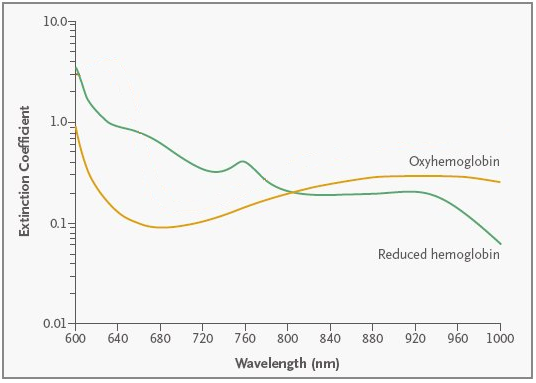
\includegraphics[width=.55\linewidth]{hemoglobin}
  \caption{Light spectrum characteristics of HbO\textsubscript{2} (oxyhemoglobin) and Hb (reduced hemoglobin).}
\end{figure}

\noindent
The arterial oxygen saturation estimate from the pulse oximeter is denoted as SpO\textsubscript{2} and is an estimate of SaO\textsubscript{2} which is defined as in the equation below.

\begin{equation}
SaO_{2} = \frac{HbO_{2}}{HbO_{2} + Hb + COHb + MetHb} \times 100 \%
\end{equation}

\noindent
The total amount of hemoglobin in the denominator of equation 2.1 is not only Hb and HbO\textsubscript{2} but also other forms of hemoglobin as carboxyhemoglobin (COHb) and methemoglobin (MetHb). The latter two are referred as dysfunctional hemoglobin because of reduced oxygen transportation and the former functional hemoglobin. A pulse oximeter uses the definition of functional oxygen saturation defined in the equation below.

\begin{equation}
SpO_{2} = \frac{HbO_{2}}{HbO_{2} + Hb} \times 100 \%
\end{equation}
\noindent
\\
The signal retrieved from the pulse oximeter is called photoplethysmographic (PPG) and is produced as a result of the periodic heart contractions and relaxation. It is a volumetric measurement associated with arterial blood volume changes. The AC part is the pulsatile component of the PPG signal related to the arterial blood volume change by cause of systolic and diastolic phases of the cardiac cycle. The DC part is the non-pulsatile component of the PPG signal associated with light intensity baseline depending on tissue, skin, bone and venous blood. The sudden drop in the systolic phase in the PPG signal is called dicrotic notch and is caused by aortic valve closure.

\begin{figure}[H]
\centering
  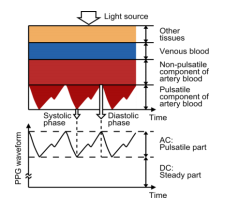
\includegraphics[width=.39\linewidth]{ppgwave}
  \caption{Light attenuation and the PPG waveform.}
\end{figure}

\noindent
The estimation of the arterial oxygen saturation and the principle of pulse oximeters is based on Beer-Lambert law. The law states that there exists an exponential relationship between the attenuation of light passing through a medium with respect to the properties of the material. The intensity of the transmitted light through the material is

\begin{equation}
\begin{split}
I = I_{0}e^{-\epsilon c l} \\
A = -ln(I/I_{0}) = \epsilon c l
\end{split}
\end{equation}


\noindent
where  \emph{I\textsubscript{0}} is the light intensity entering the volume, \emph{l} is the optical path, \emph{c} the substance concentration of the light-absorbing material and $\epsilon$ the molar absorptivity or extinction coefficient.  \emph{A} is the absorbance amount. In the case of multiple absorbers the equations become as following.

 \begin{equation}
\begin{split}
I = I_{0}e^{\sum\limits_{i}-\epsilon_{i} c_{i} l} \\
A = \sum\limits_{i} A_{i} = \sum\limits_{i} \epsilon_{i} c_{i} l
\end{split}
\end{equation}



\section{Intradialytic hypotension}

\section{Photopletysmography signal (PPG)}

\section{Optical density}

\section{Signal Processing}
\subsection{Stochastic processes}
\subsection{Stationarity, autocorrelation, mean}
\subsection{Linear Prediction}

\section{Adaptive filters}

\subsection{Least Mean Squares (LMS)}

\subsection{Normalized Least Mean Squares (NLMS)}

\subsection{Recursive Least Squares (RLS)}

\subsection{Adaptive Noise Cancellation}



\section{Optimization}
\subsection{Gradient ascent}
\subsection{Lagrange multiplier}
\subsection{Newton's method}


\section{Independent Component Analysis (ICA)}
\subsection{Definition}
\subsection{Centering}
\subsection{Whitening}
\subsection{Non-gaussianity}
\subsubsection{Kurtosis}
\subsubsection{Negentropy}


\subsection{Constrained Independent Component Analysis (cICA)}


\chapter{Method and Implementation}

\section{Material}

\subsection{CardioHolter}
\subsection{CardioLogger}

\section{Measurements}
\subsection{Synthetic data}
\subsection{Real data}

\section{Implementation of algorithms}
\subsection{First implementation}
\subsection{Second implementation}

\chapter{Results}

\chapter{Discussion}




 \renewcommand\bibname{References}
 \begin{thebibliography}{1}

  \bibitem{ref1} names. Title. {\em journal/place}, date etc.





  \end{thebibliography}








\end{document}